\documentclass[12pt]{article}
\usepackage{graphicx}
\usepackage{epstopdf}
\usepackage{lscape}
\usepackage{xcolor}
\DeclareGraphicsExtensions{.pdf,.jpeg,.png}

\usepackage{pgfplots}


\title{Estimation Results}
\author{Fieler, Orraca}
\date{\today}


\begin{document}
\maketitle
\normalsize

This document presents results for 6 different alternatives of models: alternating eta and manually multiplying the elasticity of skill intensity with respect to sales by 10 to give more importance to this moment since I had not been able to replicate it. 

I thus have 6 versions:

Model 1: $\eta=1.6$, no reweighting of any moment\\
Model 2: $\eta=1.6$, weight of $\delta_1$=10\\
Model 3: $\eta=2$, no reweighting of any moment\\ 
Model 4: $\eta=2$, weight of $\delta_1$=10\\
Model 5: $\eta=4$, no reweighting of any moment \\
Model 6: $\eta=4$, weight of $\delta_1$=10\\
\begin{landscape}
\begin{center}
{\bf Estimated parameters} \\
\begin{tabular}{ c c c c c c c c c c c } \hline
& \multicolumn{5}{c}{Non-export-oriented} & \multicolumn{5}{c}{Export-oriented}\\
& \multicolumn{5}{c}{industries} & \multicolumn{5}{c}{industries} \\  
Model & 1 & 3 & 4 & 5 & 6 & 1 & 3 & 4 & 5 & 6 \\ \hline \hline \bigskip
 $\varsigma$ & 2.15 & 2.11 & 4.35 & 1.19 & 1.56 & 0.66 & 2.35 & 2.73 & 1.11 & 1.70 \\ \bigskip 
 $\beta_l$ & 0.159 & 0.145 & 0.100 &0.283 & 0.257 & 0.229 & 0.186 & 0.219 & 0.155 & 0.171 \\  \bigskip
$\beta_h$ & 0.694 & 0.65 &0.451 &0.0824 & 0.256 & 0.842 & 0.604 & 0.322 & 0.671 & 0.215 \\ \bigskip
$a$ & 9.69 & 9.16 & 13.7 & 5.49 & 9.70 & 6.96 & 8.16 & 11.9 & 9.67 & 10.8 \\ \bigskip
$\alpha_h$ & 0.618 & 0.508 & 0.180 & 0.970 & 0.516 & 0.456 & 0.342 & 0.192 & 0.521 & 0.553 \\ \bigskip
$R_l^ *$ &2,126 & 2,285 & 1,107 & 41 & 2,635 &2,286 & 268 & 1,218 & 2,228 & 1,476 \\ \bigskip
$R_h^ *$ & 360 & 151 & 0 & 0 & 9,494 & 4,236 & 0 & 146 & 6,056 & 4,782 \\ \bigskip
$f_L$ & 675 & 778 & 773 & 4.6 & 887 & 408 & 108 & 553 & 570 & 474 \\ \bigskip
$f_X$ & 8,133 & 10,945 & 15,022 & 1,039 & 8,179 & 3,502 & 1,481 & 3,539 & 2,367 & 1,846 \\ \bigskip
$f_H$ & 1333170 & 80455 & 11380 & 114960 & 230880 & 23330 & 650 & 6710 & 39550 & 39600 \\ \hline
\end{tabular}
\end{center}
\end{landscape}

\pagebreak
\footnotesize
\begin{landscape}
\begin{center}
{\bf Model fit} \\
\begin{tabular}{ l c c c c c c c c c c c c  } \hline
& \multicolumn{6}{c}{Non-export-oriented} & \multicolumn{6}{c}{Export-oriented} \\
& \multicolumn{6}{c}{industries} & \multicolumn{6}{c}{industries} \\ 
& Data & \multicolumn{5}{c}{Model} & Data & \multicolumn{5}{c}{Model} \bigskip \\ 
& & 1 & 3 & 4 & 5 & 6 & & 1 & 3 & 4 & 5 & 6 \\ \hline \hline  
Elasticity of skill intensity wrt sales & 0.0698& 0.017  & 0.0283 &0.0698 &0.0698 &0.0698 & 0.055 & 0.007 & 0.042 & 0.055 & 0.014 & 0.055 \\ 
(non exporters) & & & & \bigskip  \\ 
 Skill intensity non-exporters & 0.062 & 0.067 & 0.062 & 0.113 & 0.059 & 0.052 & 0.097 & 0.078 & 0.097 & 0.128 & 0.015 & 0.041 \bigskip \\  \bigskip
Skill intensity exporters & 0.656 & 0.656 & 0.656 & 0.656 & 0.656 & 0.656 & 0.373 & 0.373 & 0.373 & 0.373 & 0.373 & 0.373 \\ \bigskip
$\frac{\mbox{mean domestic sales}}{\mbox{s.d. domestic sales}} $ &0.026 & 0.026 & 0.026 &0.024 & 0.012 & 0.040 & 0.048 & 0.048 & 0.012 & 0.043 & 0.057 & 0.040 \\  \bigskip
$\frac{\mbox{Domestic sales non-exporters}}{\mbox{Domestic sales exporters}} $ & 0.006 & 0.003 & 0.004 & 0.005 & 0 &0.004 & 0.012 & 0.012 & 0.003 &0.018 & 0.013 & 0.010 \\ \bigskip
Exporters' average export intensity & 0.281 & 0.273 & 0.274 & 0.281 & 0.281 & 0.272 & 0.302 & 0.302 & 0.307 & 0.298 & 0.301 & 0.299  \\ \bigskip
Elasticity of $\frac{\mbox{Foreign sales}}{\mbox{Domestic sales}}$ w.r.t. $\frac{s}{u}$ & -0.42 & -0.42 &-0.422 & -0.331 & 2.53 & -0.42 & -0.338 & -0.343 & -0.273 & -0.337 & -0.341 & -0.338  \\ \bigskip
Fraction of firms that produce (\%)\footnote{Matched by construction} & 90\footnote{Unobserved variable, target 90\%} & 90 & 90 & 90 & 90 & 90 & 90 & 90 & 90 & 90 & 90 & 90 \\ \bigskip
Export participation  (\%)\footnote{Matched by construction} & 0.59 & 0.59 & 0.59 & 0.59 & 0.59 & 0.59 & 1.7 & 1.7 & 1.7 & 1.7 & 1.7 &  1.7 \\ \bigskip
Exporters prod high skilled task (\%)\footnote{Matched by construction. In data the moment corresponds to fraction of exporters that invest in creation of new products. }  & 53.6 & 53.6 & 53.6 & 53.6 & 53.6 & 53.6 & 54.6 & 54.6 & 54.6 & 54.6 & 54.6 &  54.6 \\ \bigskip
Total difference & &0.061 & 0.044 & 0.054 & 0.022 & 0.026 & & 0.067 & 0.058 & 0.043 & 0.133 & 0.067 \\ \bigskip
Total $\frac{S}{U}$ & 0.25 & 0.476 & 0.648 & 0.477 & 0.773 & 0.449 & & & & & & \\ \hline
\end{tabular}
\end{center}
\end{landscape}

{\color{red}"Sacrifice" of matching skill intensity of low skill task is not matching elasticity of sales to skill, plus much further in $\frac{S}{U}$}



\centering
%\includegraphics[width=0.85\textwidth]{gr_XshareModel_Eta2_SinModifPesos.png}\\ 
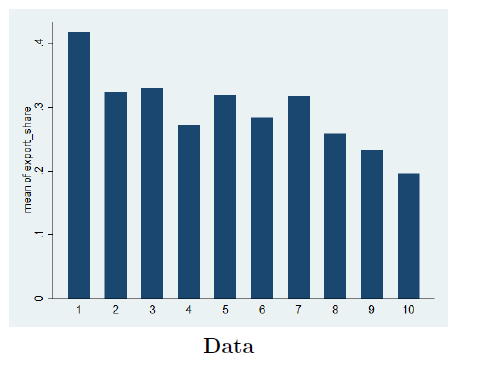
\includegraphics[width=1.0\textwidth]{DataXShareSkin.png}
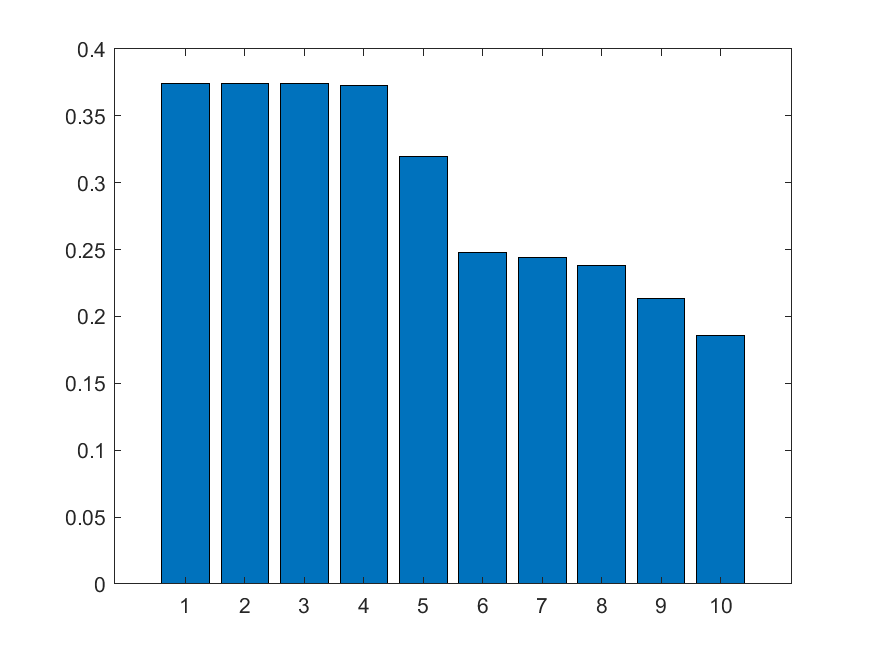
\includegraphics[width=1.0\textwidth]{grXSh_bySkint_modd1.png}


\raggedright
\pagebreak
{\bf Step \# 13:}\\
I am after $P^*_{k_j}$, whhich is the price of foreign firms selling in domestic market. This does not correspond to foreign price (so estimated $R_{k_j}^*$ above is not informative of this price). However, this price will be required in order to perform the counterfactual analysis because as $\tau$ changes, so is going to change $P_{k_j}^*$.\\ \bigskip

Estimating this moment is not simple since the imports by task are not observable (actually imports by sector are not observable either). \\ \bigskip

To get around this, we will use approximation of imports (either total imports/total manufacturing production in the whole economy, and assume that this is constant in all sectors). \\ \bigskip

For the rest of this section denote the observed price index in an industry as $P_{k_h}$; the price index of foreign firms selling in the domestic market as $P^*_{k_h}$; and domestic price index in the domestic market as $P^d_{k_h}$. 
The important thing to realize is that part of the point of this paper is comparative advantage, which implies that  $\frac{P^*_{k_h}}{P^d_{k_h}} < \frac{P^*_{k_l}}{P^d_{k_l}}$.

Revenue of firm $(k,\varphi)$ FROM TASK $k_j$ performing task $k_j$ is:
$$\alpha_{k_j}\bar{R_k}\bar{P}_{k_j}^{\sigma-1}p(\beta_{k_j},\varphi)^{1-\sigma}$$
where $\bar{R_k}$ is total domestic absorption, ie, total sales of all firms in sector $k$ (domestic and foreign sales)????? NO ME QUEDA TAAAAN CLAROOOO!!, and $\bar{P}_{k_h}$ is the final price index observed in task $k_h$, that is including foreign firms selling in domestic market. \\

LO QUE APRENDI ES QUE YO TENGO DOMESTIC SALES TOTALES DE TOOOODO EL SECTOR, NO DEL TASK, QUE ES LO QUE QUIERO, LOS PRECIOS RELATIVOS DEL TASK. ENTONCES VOY A NECESITAR LA SUMA DE LOS DOS TASKSL. REVISAR ESTO MAÑANA!!!\\

But since $P_{k_j}=\left ( \int_\omega p(\omega) ^{1-\sigma} \partial \omega \right)^{\frac{1}{1-\sigma}}$, then we can say that $P_{k_j}^{1-\sigma}=P_{k_j}^{1-\sigma}+P_{k_j}^{*1-\sigma}$, which means that $\bar{P}_{k_j}^{\sigma-1}=\frac{1}{P_{k_j}^{1-\sigma}+P_{k_j}^{*1-\sigma}}$. Thus,
$$r(\beta_{k_h},\varphi)=\alpha_{k_j}\bar{R_k}\bar{P}_{k_j}^{\sigma-1}p(\beta_{k_j},\varphi)^{1-\sigma}=\alpha_{k_j}\bar{R_k}\frac{p(\beta_{k_j},\varphi)^{1-\sigma}}{P_{k_j}^{1-\sigma}+P_{k_j}^{*1-\sigma}}$$ 
Doing some manipulation,
$$r(\beta_{k_h},\varphi)=\alpha_{k_j}\bar{R_k}\frac{P_{k_j}^{1-\sigma}}{P_{k_j}^{1-\sigma}+P_{k_j}^{*1-\sigma}}\frac{p(\beta_{k_j},\varphi)^{1-\sigma}}{P_{k_j}^{1-\sigma}}$$
Then, summing over all firms to get total revenue of task $k_j$:
$$\alpha_{k_j}\bar{R_k}\frac{P_{k_j}^{1-\sigma}}{P_{k_j}^{1-\sigma}+P_{k_j}^{*1-\sigma}} \frac{1}{{P_{k_j}^{1-\sigma}}}\int p(\beta_{k_j},\varphi)^{1-\sigma}=\alpha_{k_j}\bar{R_k}\frac{1}{P_{k_j}^{1-\sigma}+P_{k_j}^{*1-\sigma}} \int p(\beta_{k_j},\varphi)^{1-\sigma}$$
But again $\int p(\beta_{k_j},\varphi)^{1-\sigma}=P_{k_j}^{1-\sigma}$, so we conclude
$$Total sales task k_j=\alpha_{k_j}\bar{R_k}\frac{P_{k_j}^{1-\sigma}}{P_{k_j}^{1-\sigma}+P_{k_j}^{*1-\sigma}} $$



\end{document}
